\chapter{Aspectos Técnicos}\label{chapter:technical}

En este capítulo se describen los aspectos técnicos necesarios para comprender el diseño e implementación del proyecto. Primero, se presentan los componentes de software y hardware utilizados. Luego, se revisan algoritmos y conceptos computacionales utilizados en el trabajo.

%% =============================================================================

%% =============================================================================

%% =============================================================================

%% =============================================================================

%% =============================================================================

%% =============================================================================
%% =============================================================================
%% =============================================================================
\section{Componentes de software y hardware}
%% =============================================================================
%% =============================================================================
%% =============================================================================

A continuación se describen los componentes de software y hardware utilizados para el diseño e implementación del proyecto: Se hace una revisión breve de la base de datos MongoDB. Se revisan los conceptos utilizados sobre el framework robótico ROS. Se describe la librería SMACH, utilizada para la creación de máquinas de estado. Y finalmente, se presenta a Bender junto a los aspectos requeridos de su sistema operativo.

%% =============================================================================
%% =============================================================================
%% =============================================================================
\subsection{ROS}
%% =============================================================================
%% =============================================================================
%% =============================================================================

ROS \cite{ROS:2009}, acrónimo para Robot Operating System, es un proyecto que funciona como \textit{middleware} para aplicaciones robóticas, y permite resolver el problema de la comunicación entre procesos. Es una colección de herramientas, librerías y convenciones que buscan simplificar la tarea de crear comportamientos robóticos complejos y robustos, sin importar la plataforma robótica.

Fue originalmente creado por la organización WillowGarage en el 2008, y es mantenido actualmente por la Open Source Robotics Foundation (OSRF). Existe un ecosistema ROS, mantenido por la comunidad, y con cientos de módulos de software con soluciones a problemas específicos, los que pueden interconectarse para construir comportamientos más complejos. Por lo anterior, su uso se ha convertido en una práctica mundial, siendo adoptado incluso en soluciones industriales.

\todounsure{Agregar diagramas funcionamiento ROS??.. }

\subsubsection{Intraestructura}
%% =============================================================================

\paragraph{Nodo}
Es un programa ejecutable en ROS, enfocado en una tarea específica. Cada nodo puede establecer comunicación con otros a través de una interfaz ROS de tópicos o servicios.

\paragraph{Paquete}
Corresponde a un conjunto de nodos, junto a todos sus archivos necesarios para su compilación y ejecución. Cada paquete tiene asociado un nombre único en el sistema, junto a una lista de dependencias de otros paquetes. ROS provee conjunto estándar de paquetes y librerías enfocados en diversos aspectos de la robótica, que en conjunto a los paquetes mantenidos por la comunidad, permiten simplificar la construcción y mantenimiento de un robot.

\paragraph{Distribuciones} 
Una distribución es un conjunto versionado de paquetes ROS. Su propósito es permitir que los desarrolladores trabajen en un conjunto relativamente estable de dependencias, hasta que puedan avanzar a la siguiente versión. Se libera una distribución anualmente, enfocada a una versión  LTS\footnote{LTS es un acrónimo para Long-Term-Support. Una versión LTS de un software indica que éste contará con soporte a largo plazo, es decir, durante un periodo mayor a su periodo normal de vigencia.} de Ubuntu, y las versiones pares de ROS también se consideran LTS y mantienen soporte por 5 años.

\paragraph{Lenguajes de programación} ROS provee librerías oficiales para escribir nodos en los lenguajes C++ (\texttt{roscpp}\footnote{Documentación oficial de \texttt{roscpp}: \url{http://wiki.ros.org/roscpp}.}), Python (\texttt{rospy}\footnote{Documentación oficial de \texttt{rospy}: \url{http://wiki.ros.org/rospy}.}) y Common Lisp (\texttt{roslisp}\footnote{Documentación oficial de \texttt{roslisp}: \url{http://wiki.ros.org/roslisp}.}), junto a librerías experimentales para otros lenguajes.

\subsubsection{Comunicación}
%% =============================================================================

\paragraph{ROS master} Es el servidor central de ROS y provee servicios de registro al resto de los nodos. Mantiene una lista de los tópicos, servicios y parámetros disponibles, que han registrado los nodos activos. Su principal funcionalidad es permitir que cada nodo pueda encontrar a los otros. Una vez establecida la comunicación, los nodos se comunican en una red P2P\footnote{En una red P2P (peer-to-peer) los participantes se comunican total o parcialmente sin requerir un servidor intermediario.}. Comúnmente la comunicación en ROS se realiza mediante el protocolo HTTP, bajo un transporte TCP, sin embargo, los nodos pueden ser configurados para utilizar un transporte basado en UDP. Por lo tanto, ROS permite el manejo de nodos de manera distribuida, siempre que cada máquina tenga acceso a la red del computador ejecutando el ROS master.

\paragraph{Mensaje} Es una estructura de datos utilizada para comunicar un nodo con otro. Se definen en un mensaje de tipo \texttt{.msg}, a partir de tipos de dato básicos en ROS y otros mensajes. Durante la compilación se generan el código para poder utilizarlos mediante las librerías ROS de cada lenguaje de programación disponible.

\paragraph{Tópico} Permite que los nodos de comuniquen a través de mensajes, y está basado en el patrón de diseño observador. Cada tópico es un canal de comunicación que transmite mensajes ROS de un tipo predefinido. Cada nodo puede publicar simultáneamente en uno o más tópicos. Cada nodo puede suscribirse a los tópicos que desee, siendo notificado por cada mensaje entrante. Esto se describe en el diagrama de la Figura \ref{img:ros-topic}.

\begin{figure}[!h]
	\centering
	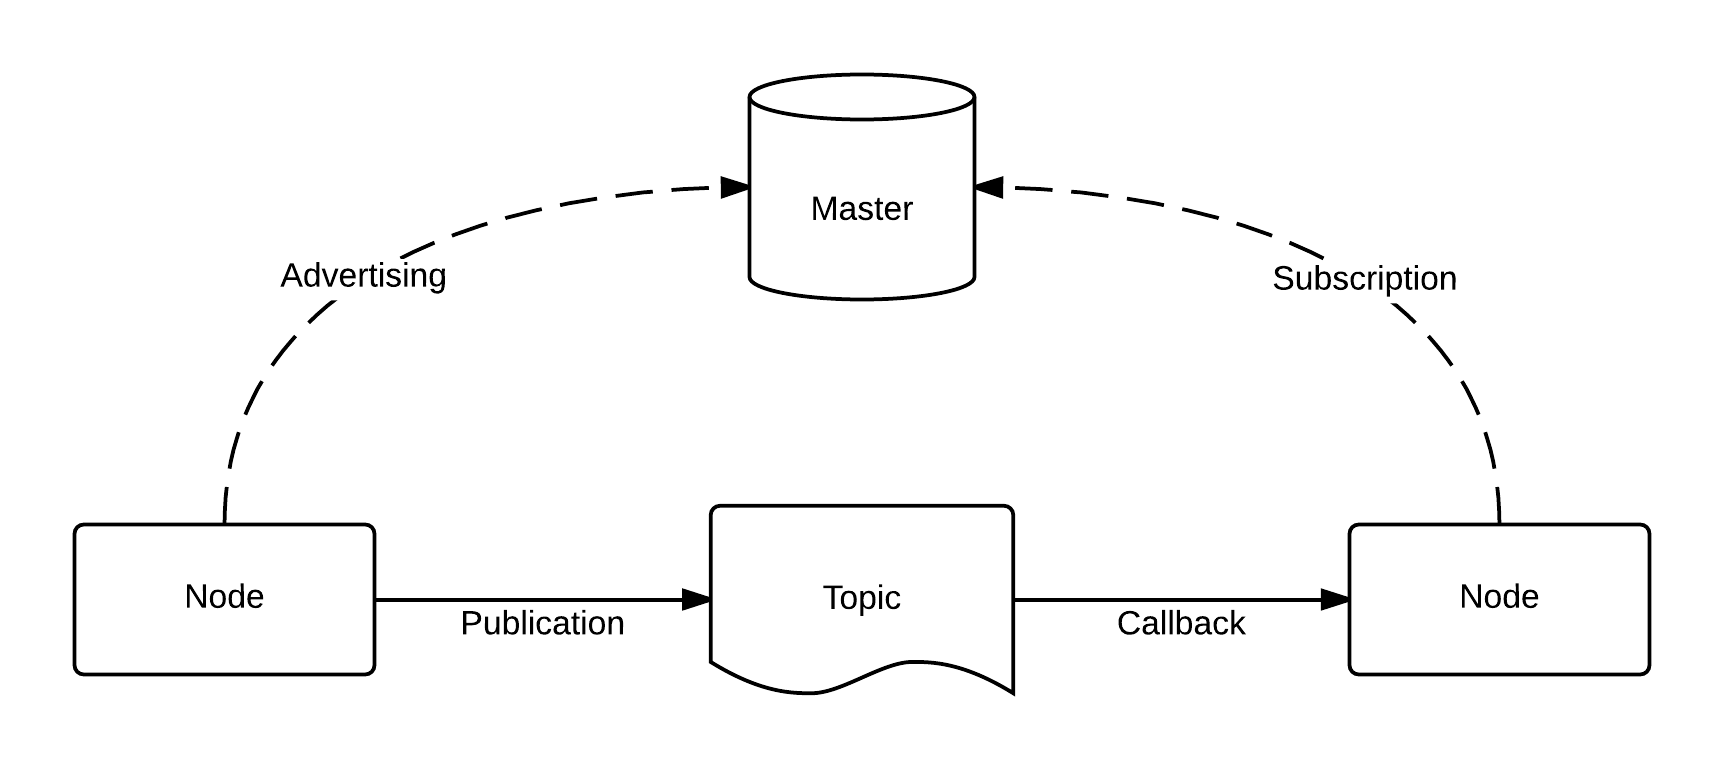
\includegraphics[width=0.8\textwidth]{ROS-master-node-topic.png}
	\caption{\small Diagrama de la comunicación mediante tópicos en ROS. El ROS master se encarga de establecer iniciar el proceso de comunicación entre los nodos involucrados. Luego los nodos se comunican {\bfseries unidireccionalmente} usando el tópico establecido.}
	\label{img:ros-topic}
\end{figure}
\todoimprove{Figura en español.}

\paragraph{Servicios} Es una forma de comunicación cliente-servidor, de carácter síncrono. Se construyen a partir de una estructura de datos de tipo \texttt{.srv}, que especifica mensajes ROS de petición y respuesta, disponible tras la compilación. Cada nodo (servidor) puede proveer uno o más servicios. Cada nodo (cliente) puede enviar peticiones al servidor. Las peticiones son de carácter bloqueante, hasta que una respuesta desde el servidor sea recibida.

\paragraph{Acciones} Esta forma de comunicación se construye a partir de tópicos y servicios, mediante la librería \texttt{actionlib} \footnote{Documentación oficial de \texttt{actionlib}: \url{http://wiki.ros.org/actionlib}.}. Está enfocada en la resolución de tareas de largo plazo, y funciona a través de metas solicitadas por el cliente. El servidor mantiene una máquina de estados que recibe peticiones (servicio) e informa constantemente sobre el estado del proceso y su resultado (tópicos). La estructura de datos utilizada es de tipo \texttt{.action}, que especifica mensajes ROS para la petición, el \textit{feedback} y el resultado.

\paragraph{Servidor de parámetros} ROS provee un servidor para almacenar, modificar y obtener parámetros compartidos entre los nodos. Éstos permiten la configuración del programa sin tener que recompilar el código, y funcionan como el estándar para el manejo de parámetros. La configuración por defecto puede ser especificada en archivos en formato YAML.



\subsubsection{Herramientas}
%% =============================================================================

\paragraph{Pluginlib} Es un paquete oficial de ROS\footnote{Documentación oficial de \texttt{pluginlib}: \url{http://wiki.ros.org/pluginlib}.} que provee herramientas para escribir y cargar plugins dinámicamente en C++. La librería permite delegar la implementación de funcionalidades específicas a los usuarios. El nodo que ocupará el plugin debe definir una clase abstracta a ser implementada. Mientras que los paquetes proveedores deben registrar las librerías con sus implementaciones, para que los plugins queden disponibles en el sistema.

\paragraph{Roslaunch} La librería \texttt{roslaunch}\footnote{Documentación oficial de \texttt{roslaunch}: \url{http://wiki.ros.org/roslaunch}.} es una herramienta que permite la ejecución y configuración de múltiples nodos, a través de sólo un comando en la consola del sistema. Utiliza archivos en formato XML y con extensión \texttt{.launch}, para definir un árbol de nodos y otros archivos \textit{launch} a ser ejecutado. Esta herramienta permite modularizar la ejecución de un sistema robótico complejo, compuesto generalmente por decenas de nodos.

%\paragraph{Rviz}
%\paragraph{Rosbag} (probablemente se ocupará para test suite)


%% =============================================================================
%% =============================================================================
%% =============================================================================
\subsection{MongoDB}
%% =============================================================================
%% =============================================================================
%% =============================================================================

\subsubsection{Conceptos:}

MongoDB es una base de datos no relacional orientada a documentos tipo JSON, donde los campos pueden variar de documento a documento y la estructura de datos puede ser modificada en el tiempo \cite{MongoDB}. MongoDB está diseñada para funcionar de manera distribuida, proveer alta disponibilidad, escalamiento horizontal y distribución geográfica. Es una base de datos gratis y de código libre, publicada bajo la licencia GNU AGPL.

MongoDB representa documentos JSON en un formato binario denominado BSON. BSON extiende JSON a través de nuevos tipos de datos, campos ordenados y para proveer eficiencia al codificar y decodificar la información en distintos lenguajes. 

Los documentos son organizados en \textit{colecciones}, cada una destinada a almacenar información asociada a un concepto particular. MongoDB provee funcionalidades para consultas, indexado y realizar agregaciones de los datos almacenados.

MongoDB provee drivers para diversos lenguajes de programación, entre ellos C++, Java y Python. Para este proyecto, el driver de interés es el de C++11\footnote{Documentación del driver de MongoDB para C++:  \url{http://mongodb.github.io/mongo-cxx-driver/}.}.

En su configuración por defecto, el servidor de MongoDB soporta documentos de hasta 16MB de tamaño, lo que restringe la información a almacenar, pero permite mantener acotados los costos de las operaciones sobre la base de datos. El límite puede ser removido al modificar el algoritmo de almacenamiento a GridFS, que divide documentos grandes en subdocumentos menores a 16MB, para ser tratados normalmente.

\subsubsection{Interfaz ROS:}

MongoDB es una de las dependencias de \textit{MoveIt!}\footnote{Documentación oficial de MoveIt!: \url{https://moveit.ros.org/}.}, librería estándar utilizada para la manipulación de objetos, de uso extendido en la comunidad robótica. Por lo tanto, MongoDB ya está instalada y funcionando en muchos robots de servicio basados en ROS. 

El equipo desarrollador de MoveIt! y sus paquetes ROS relacionados mantiene el paquete \texttt{warehouse\_ros\_mongo}\footnote{El paquete ROS \texttt{warehouse\_ros\_mongo} está disponible en: \url{https://github.com/ros-planning/warehouse\_ros\_mongo}.}, que provee una interfaz ROS al driver en C++ para MongoDB. MoveIt! y sus dependencias son consideradas estables, al menos durante el periodo de la última distribución ROS, con fecha de caducidad para el 2023.

\texttt{warehouse\_ros\_mongo} permite definir colecciones destinadas a almacenar mensajes ROS, de manera binaria. Cada documento es construido a partir del mensaje ROS serializado (mediante su API ROS), sumado a un conjunto de metadatos utilizados para la definición de índices y consultas. Actualmente, la API sólo soporta la definición de metadatos de los tipos \texttt{bool}, \texttt{int}, \texttt{double} y \texttt{std::string} en C++.


%% =============================================================================
%% =============================================================================
%% =============================================================================
\subsection{SMACH}
%% =============================================================================
%% =============================================================================
%% =============================================================================

SMACH es una librería en Python para la creación y ejecución de máquinas de estado. Permite crear rápidamente comportamientos robóticos complejos, basados en capacidades de alto nivel de un robot. Está diseñada para ser independiente de ROS, pero provee una interfaz para su uso. Se puede encontrar en el conjunto de paquetes ROS denominado \texttt{executive\_smach}\footnote{Documentación oficial de SMACH disponible en: \url{http://wiki.ros.org/smach}.}.

\begin{figure}[!h]
	\centering
	\includegraphics[width=0.8\textwidth]{smach-sample.png}
	\caption{\small Ejemplo de máquina de estado construida en SMACH para la representación de una rutina de carga automática de baterías. Obtenido desde la documentación oficial.}
	\label{img:SMACH-sample}
\end{figure}
\todoimprove{Figura en español}


En SMACH una maquina de estado está compuesta por un conjunto de estados y sus transiciones. Las La librería soporta el anidamiento, por lo que cualquier estado puede ser reemplazado por otra máquina de estado disponible. Cada estado debe proveer una función \texttt{execute} a ser ejecutada cuando esté activo. En la Figura \ref{img:SMACH-sample} se presenta un ejemplo de un comportamiento robótico complejo implementado en SMACH, que representa el proceso de recarga de baterías en un robot. Según las condiciones encontradas se activarán distintas transiciones, pero en el caso básico la rutina es la siguiente: Robot navega a la estación de carga, se posiciona, manipula el conector, se conecta y espera.

%% =============================================================================
%% =============================================================================
%% =============================================================================
\subsection{UChile ROS Framework}
%% =============================================================================
%% =============================================================================
%% =============================================================================

\subsubsection{Conceptos}

UChile ROS Framework (URF) hace referencia al sistema de software desarrollado en el laboratorio de robótica del Departamento de Ingeniería Eléctrica de la Universidad de Chile, para sus robots de servicio. El sistema cuenta con 10 años de desarrollo y está orientado a cumplir los requisitos de la competencia RoboCup en su categoría @Home.

URF está construido sobre ROS y en una estructura de 4 capas:
\begin{enumerate}
\item La primera capa contiene todas las dependencias del sistema, ya sean de ROS o no. Es la única capa que contiene sólo código externo.
\item  Sobre la primera capa se monta una capa ROS de bajo nivel, con herramientas y librerías comunes, sumado a los drivers necesarios para manejar cada robot (módulos de \textit{Hardware} en la Figura \ref{img:URF}).
\item La capa intermedia alberga capacidades robóticas avanzadas, relacionadas a percepción robótica, manipulación de objetos, navegación autónoma e interacción Humano-Robot (sección \textit{ROS modules} del diagrama).
\item La última capa \textit{de alto nivel} es desarrollada en Python, con interfaces para el uso de las capacidades de menor nivel, y utilizada para la elaboración de maquinas de estado y comportamientos robóticos complejos mediante SMACH (cuadros \textit{ROS-python interface} y \textit{State Machine} del diagrama).
\end{enumerate}

\begin{figure}[!h]
	\centering
	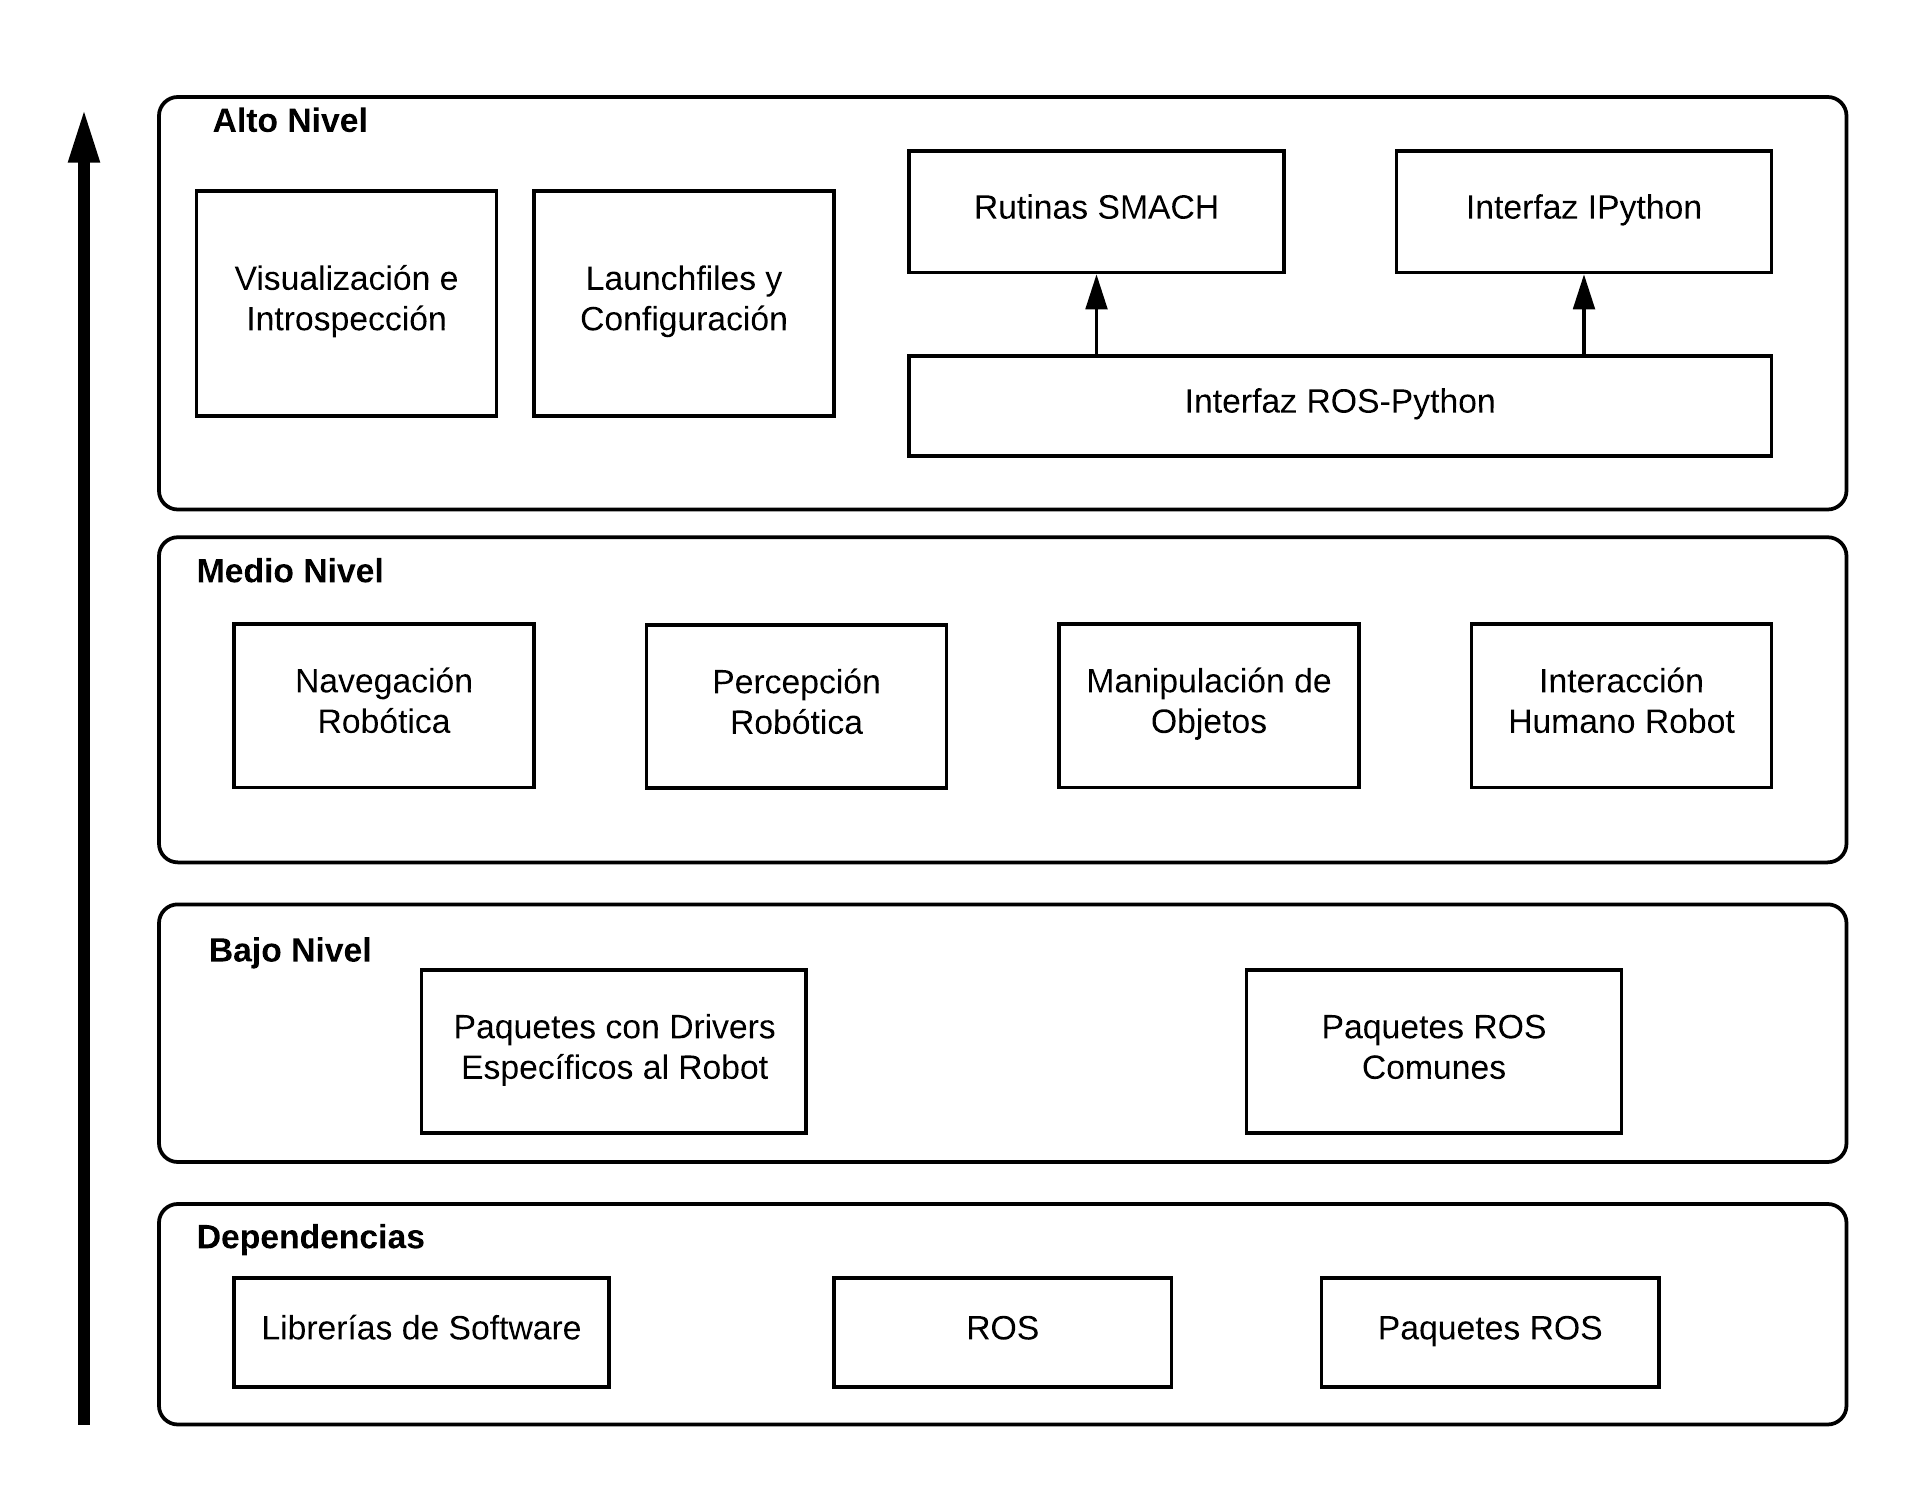
\includegraphics[width=0.8\textwidth]{URF.png}
	\caption{\small Diagrama de UChile ROS Framework utilizado en el robot Bender.}
	\label{img:URF}
\end{figure}

\todoimprove{Figura en español}

Todos los módulos de URF son de código libre, a excepción de los algoritmos relacionados con percepción y la interfaz de alto nivel. El código se almacena públicamente en la organización \textit{uchile-robotics} en GitHub\footnote{Organización \textit{uchile-robotics} y URF en GitHub: \url{https://github.com/uchile-robotics}}.


\subsubsection{Memoria a corto y largo plazo}
%% =============================================================================

En un robot implementado sobre URF es posible acceder a la información compartida por sus procesos. Cualquier módulo ROS en el sistema tiene acceso a los datos extraídos desde sensores y luego generados en post-procesamientos, junto al acceso para controlar el hardware.

Existen algunas formas de memoria implementadas en URF, comparables a los conceptos definidos para la memoria humana. También se pueden dividir en de corto y largo plazo:

Como STM, se puede definir como memoria de trabajo a todo el flujo de información presente durante la ejecución del robot. Lo que incluye datos sensados, procesamientos y acciones realizadas. Generalmente tales datos no son almacenados para posteriores ejecuciones.

A manera de LTM, se puede encontrar una memoria procedural, relacionada con todo el conocimiento almacenado que posee el robot para cumplir ciertas tareas. Caen en esta categoría: modelos para percepción robótica, modelos para reconocimiento de voz y patrones, bases de datos de movimientos precalculados para manipular objetos y acciones predefinidas que se utilizan para controlar el robot.

También se pueden encontrar especializaciones de memoria LTM semántica. Ejemplos de esto son: El mapa que se conoce del entorno, junto a los lugares y objetos anotados en él. Diccionarios con información anotada sobre entidades y sus características, cómo personas y objetos. Bases de datos con imágenes anotadas para el reconocimiento de objetos y personas. 

Sin embargo, en URF no existen formas de memoria emocional ni episódica de largo plazo. Luego, toda interacción realizada por los robots está limitada a la información obtenida desde el inicio al término de cada rutina.


%% =============================================================================
%% =============================================================================
%% =============================================================================
\subsection{Bender}
%% =============================================================================
%% =============================================================================
%% =============================================================================
%% -----------------------------------------------------------------------------

Bender es un robot humanoide creado el año 2007 en el laboratorio de robótica del Departamento de Ingeniería Eléctrica de la Universidad de Chile. El equipo UChile Homebreakers es el encargado de su desarrollo y  su objetivo es ser un mayordomo para el hogar, funcionando de manera autónoma para apoyar en tales labores \cite{uchile-robotics}.

En cuanto a actuadores, el robot cuenta con 2 brazos antropomórficos de 6 grados de libertad cada uno, una base móvil diferencial Pioneer 3-AT, un cuello que permite rotaciones en dos ejes cartesianos; pudiendo imitar gestos de asentimiento y negación, y finalmente, una cabeza que puede mostrar expresiones faciales mediante movimientos de su boca, orejas, cejas y cambios de colores alrededor de los ojos.

El robot cuenta con los siguientes sensores: un laser Hokuyo UTM-30LX, un laser Hokuyo URG-04LX-UG01, un micrófono M-Audio Producer USB y una cámara de profundidad ASUS Xtion Pro.

El software de Bender está basado en el framework URF. Su arquitectura de software utiliza  ROS para el manejo de componentes de bajo y medio nivel. La capa de alto nivel, escrita en python, se abstrae de ROS y permite la creación de comportamientos complejos mediante máquinas de estado. Todos los módulos que interactúan con sensores y actuadores están implementados en ROS.

\begin{figure}[!h]
	\centering
	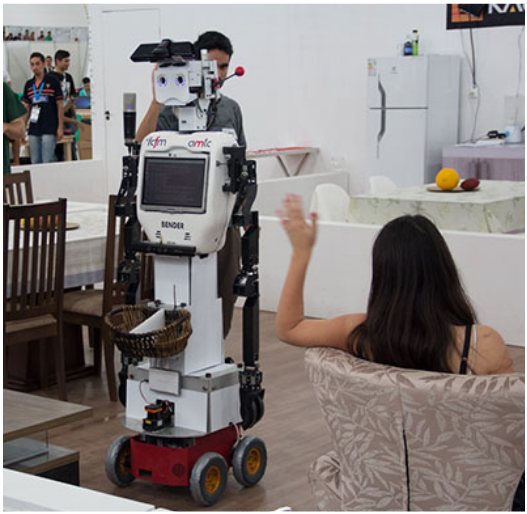
\includegraphics[width=0.5\textwidth]{bender.png}
	\caption{\small Robot Bender en competencia RoboCup@Home 2015.}
	\label{img:bender}
\end{figure}

\todoimprove{Sobre la cantidad de paquetes ROS, nodos, tópicos y mensajes disponibles.}
\todoimprove{API a ocupar para acceder a datos del robot.}


%% =============================================================================

%% =============================================================================

%% =============================================================================

%% =============================================================================

%% =============================================================================

%% =============================================================================

%% =============================================================================
%% =============================================================================
%% =============================================================================
\section{Algoritmos y conceptos computacionales}
%% =============================================================================
%% =============================================================================
%% =============================================================================

\todounsure{convex hull}
\todounsure{procesamiento de imágenes: degradación de streams}
\todounsure{Algs utilizados para emociones implementadas en robot}
\todounsure{Sistemas de coordenadas?? Frames?}



